Having evaluated the fitted surfaces, we used them to generate complete contract paths and examine how the stock and IV inputs entered American-option valuation. We selected one put and one call for each of GS and LLY from the April 28 capture with expiration on May 29 (Supplementary Tables~\ref{tab:gs_scenario} and~\ref{tab:lly_scenario}). The initial illustrations used 1{,}000 stock paths per ticker and a separate IV factor for each contract under the fixed settings in Supplementary Table~\ref{tab:scenario_settings}. Each factor followed a moving target supplied by the fitted surface before its IV entered the lattice calculation at the current stock price and remaining maturity. The GS paths showed the expected inverse relation between terminal stock and put payoff and the direct relation between terminal stock and call payoff (Fig.~\ref{fig:gs_paths}). Before expiration, the put and call factors followed different targets as moneyness and calendar days to expiration changed (Fig.~\ref{fig:gs_iv}). Their shared negative return coupling tended to increase factor shocks after lower standardized returns. The corresponding LLY paths demonstrated the same calculation under a different return marginal and higher fitted IV level (Supplementary Figs.~\ref{fig:lly_paths} and~\ref{fig:lly_iv}). The pathwise Greeks described the associated risk sensitivities through delta approaching the exercise states, gamma concentrating near the strike, and Vega declining toward expiration (Supplementary Figs.~\ref{fig:gs_greeks} and~\ref{fig:lly_greeks}). Algorithm~\ref{alg:forward_sim} describes these illustrations with return shocks standardized across the completed ensemble. The paired ablation used independent pilot constants instead, as described in Section~\ref{sec:ablation_methods}, to measure the contribution of IV dynamics on shared evaluation paths. Both experiments used surfaces fitted with observations from the scenario period and examined the behavior of the assembled model. They were illustrative scenarios, not forecasts evaluated against later observations; the chronological tests used separate fits and origins.

\begin{algorithm}[H]
\caption{Forward simulation of contract values}\label{alg:forward_sim}
\begin{algorithmic}[1]
\Require JumpHMM marginal; fitted $(\theta_i,\psi_i)$; contract $(K,T)$; trading dates $d_0,\ldots,d_L$; calendar DTE $\tau_0,\ldots,\tau_L$; $(\kappa,\sigma_v,\rho)$; $S_0$; $r$; $N_p$ paths; LR depth $N_{\mathrm{LR}}$.
\Ensure Stock, variance, IV, and option-value paths.
\State Draw $N_p$ JumpHMM stock paths with $L$ trading transitions.
\State Compute $Z^S_{j,\ell}$ by standardizing all simulated one-session log returns as in~\eqref{eq:return_shock}.
\State Draw $Z^\perp_{j,\ell}\sim\mathcal N(0,1)$ once per path and transition; set $Z^v_{j,\ell}\gets\rho Z^S_{j,\ell}+\sqrt{1-\rho^2}Z^\perp_{j,\ell}$ and reuse it for every contract.
\For{contract $a$ and path $j$}
  \State $v_{a,0}^{(j)} \gets \theta_i\psi_i(\tau_0,K/S_0)$
  \For{$\ell=0$ \textbf{to} $L-1$}
    \State $\sigma_{a,\ell}^{(j)} \gets \sqrt{v_{a,\ell}^{(j)}}$
    \State $P_{a,\ell}^{(j)} \gets \mathrm{LR}_{N_{\mathrm{LR}}}(S_{j,\ell},K,\sigma_{a,\ell}^{(j)},\tau_\ell/365,r)$
    \State $\bar v_{a,\ell}^{(j)}\gets\theta_i\psi_i(\tau_\ell,K/S_{j,\ell})$
    \State Update $v_{a,\ell+1}^{(j)}$ with the hard-floor rule in~\eqref{eq:euler} using $\Delta t=1/252$.
  \EndFor
  \State $P_{a,L}^{(j)}\gets\max\{\phi(S_{j,L}-K),0\}$, where $\phi=1$ for a call and $\phi=-1$ for a put.
\EndFor
\State \Return all paths.
\end{algorithmic}
\end{algorithm}

\begin{figure}[!htbp]
\centering
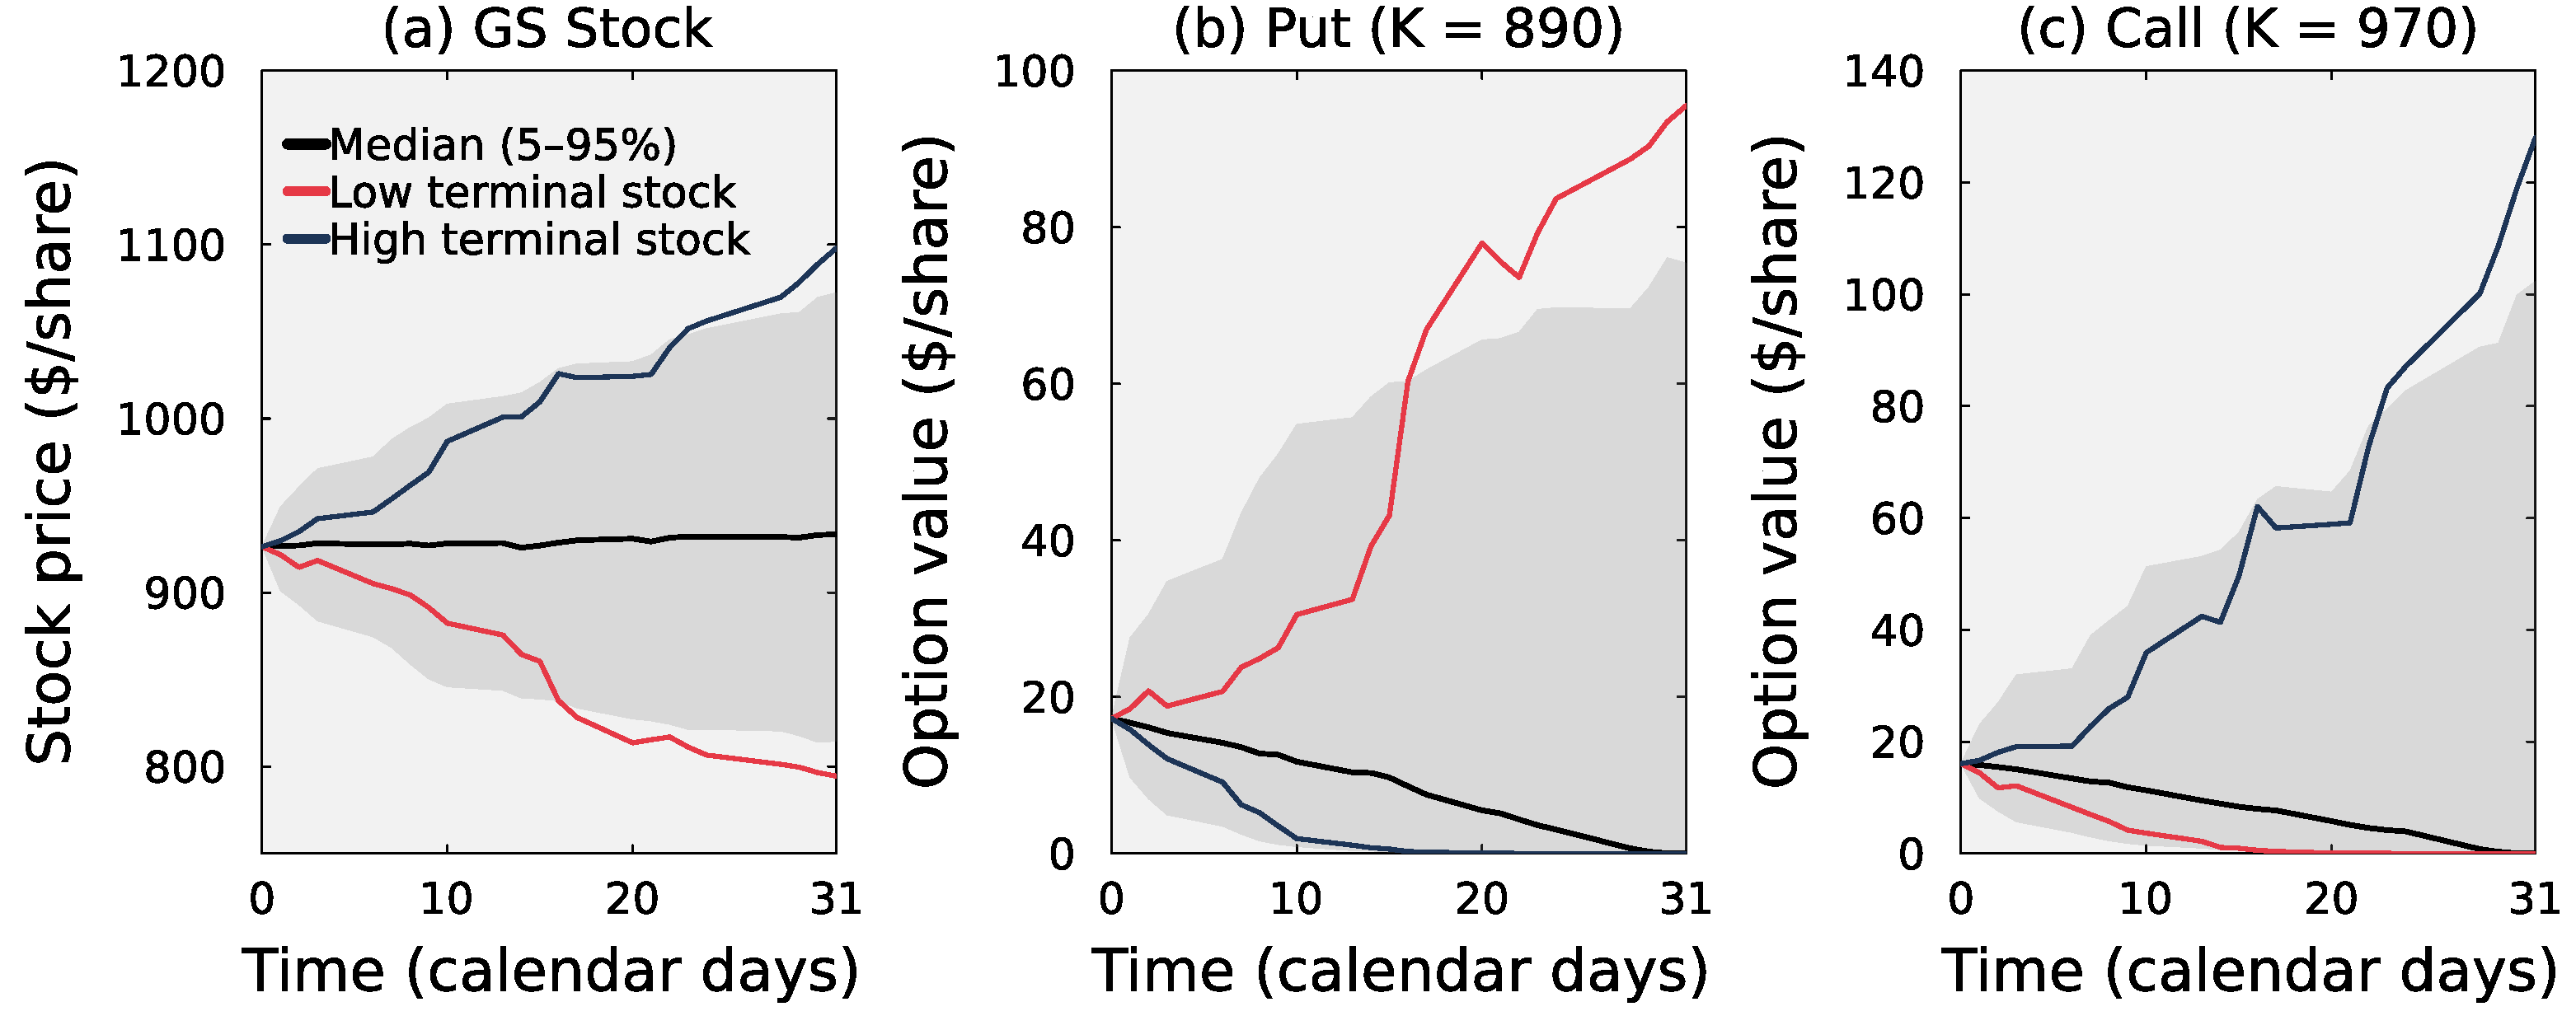
\includegraphics[width=\textwidth]{sections/figures/gs/gs_short_paths.pdf}
\caption{Simulated evolution of GS stock prices (a), put values (b), and call values (c) along 1{,}000 paths between April 28 and May 29, 2026. The fitted surfaces included observations from this scenario period, so these paths illustrate the model rather than an out-of-sample forecast. Time is measured in calendar days from April 28. Black curves show the median at each date, and shaded bands contain the middle 90\% of values. Red and blue curves show group medians for paths ranked in the 1st--5th and 95th--99th percentiles of terminal stock price. These summaries are not individual trajectories. Option values are dollars per share and represent the cost of repurchasing the contract for a short seller. Entry premiums were \$16.51 per share for the put and \$16.09 for the call.}
\label{fig:gs_paths}
\end{figure}

\begin{figure}[!htbp]
\centering
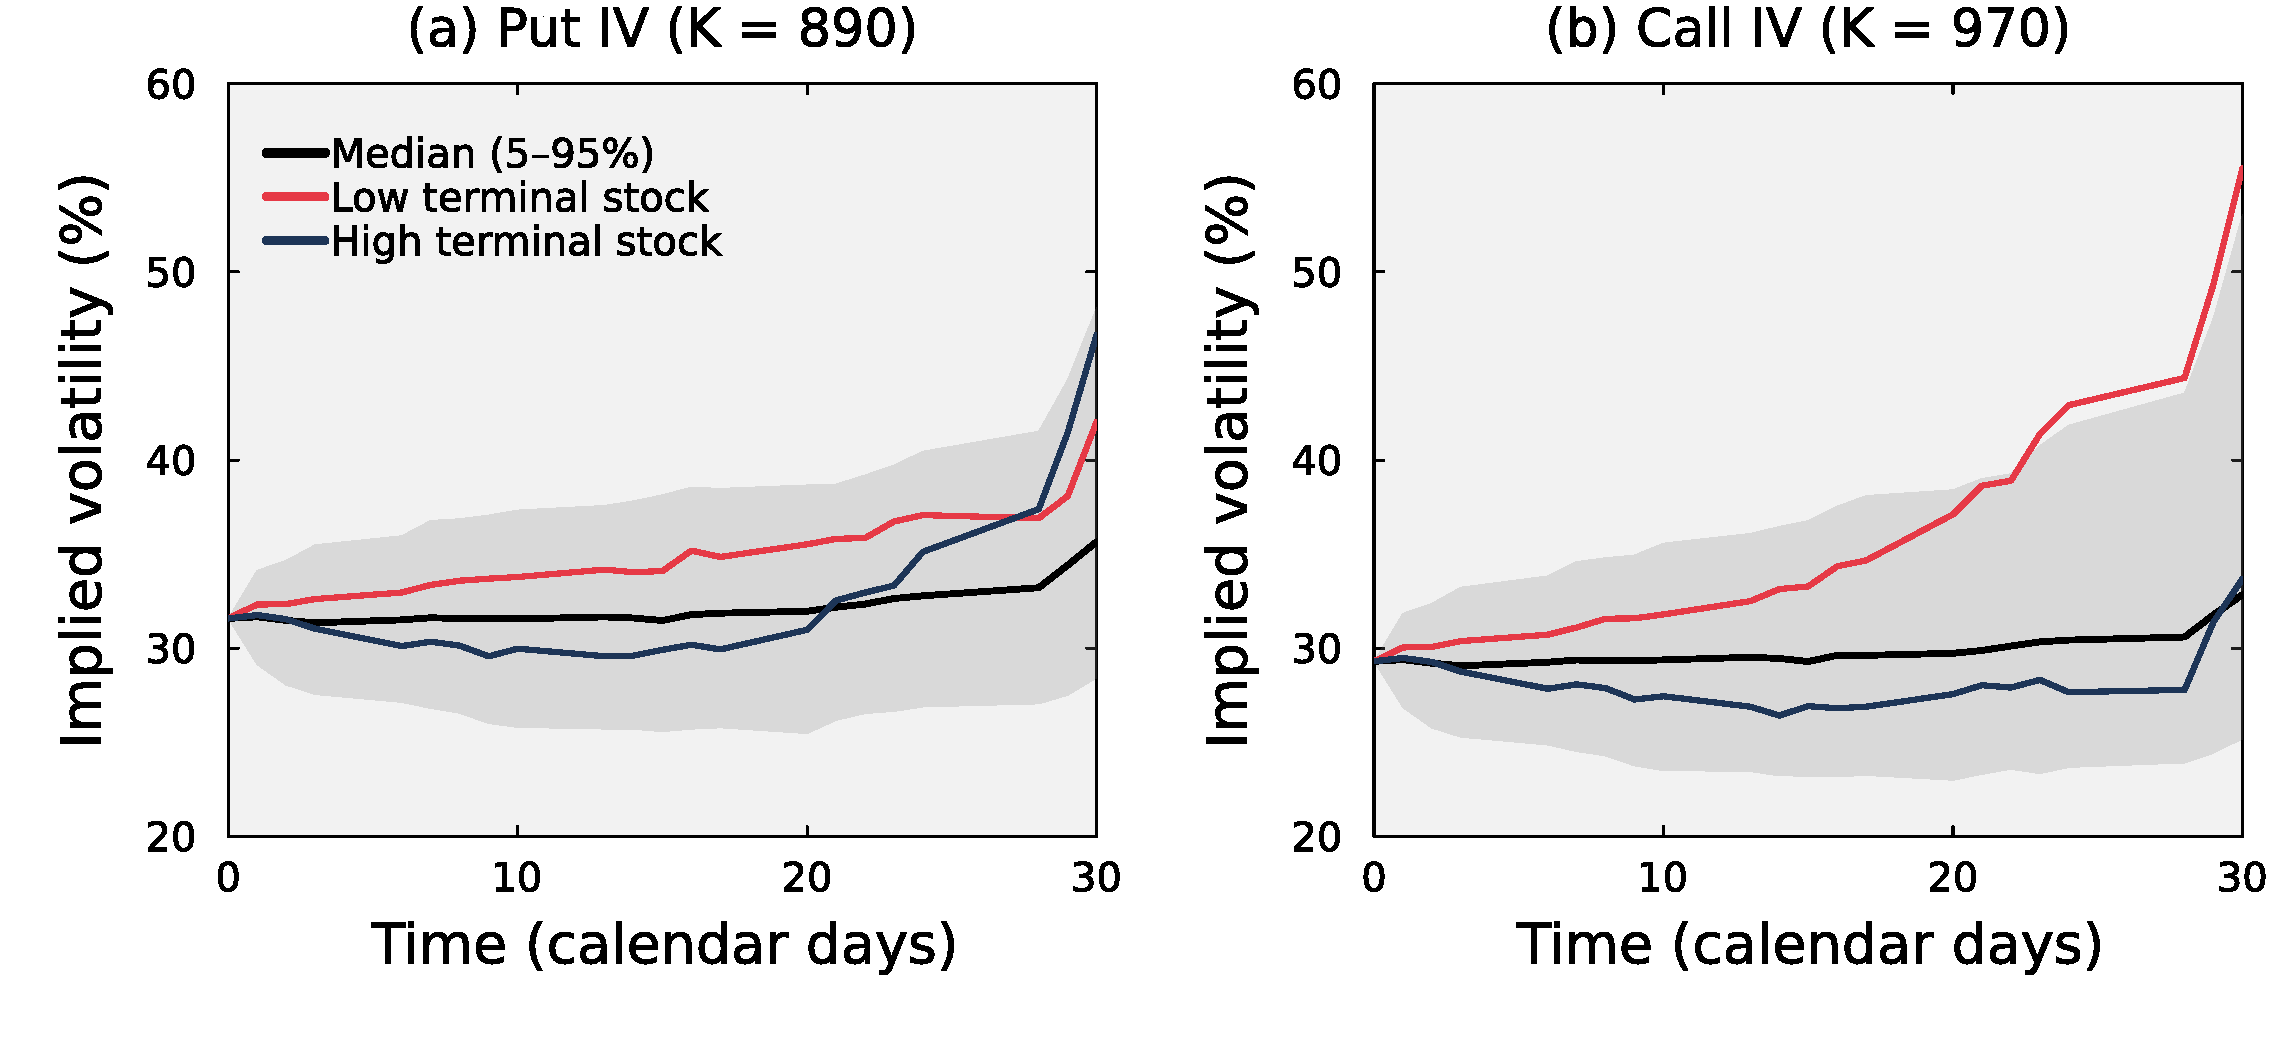
\includegraphics[width=\textwidth]{sections/figures/gs/gs_iv_trajectories.pdf}
\caption{Simulated evolution of annualized IV at the GS put strike (a) and call strike (b). These factors belong to the illustrative scenario in Fig.~\ref{fig:gs_paths}. Both panels express IV as percentages on the same vertical scale. Curves show pointwise medians across all 1{,}000 paths and within the terminal-stock groups defined in Fig.~\ref{fig:gs_paths}; shading shows the 5th--95th percentile band. Time is measured in calendar days from April 28, 2026, and stops before expiration. IV does not enter the expiration payoff.}
\label{fig:gs_iv}
\end{figure}

\FloatBarrier
To measure the contribution of IV dynamics, we compared five variants on identical stock paths for the four scenario contracts. The comparison held contracts, entry premiums, and pricing assumptions fixed so that differences in interim marks could be attributed to the IV module (Section~\ref{sec:ablation_methods}). After ten trading transitions, the full factor changed marks by a mean absolute \$1.77--\$2.41 per share relative to direct surface evaluation (Supplementary Table~\ref{tab:dynamic_ablation}). These pathwise changes were much larger than the corresponding difference in the GS put's mean P\&L, which was only \$0.05 lower under the full factor with a paired Monte Carlo standard error of \$0.04. Positive and negative differences therefore largely canceled when averaged across paths. Frozen IV and deterministic mean reversion also produced different marks from the direct surface, showing that movement of the target and persistence around it affected valuation even without stochastic shocks. Comparing the coupled and uncoupled factors on the same paths showed how return coupling changed valuation across stock outcomes. For both tickers, short-put P\&L declined most on falling-stock paths, while short-call P\&L improved most on rising-stock paths (Fig.~\ref{fig:dynamic_ablation}). Coupling also changed the lower tails of short-position P\&L. We measured those tails with 5\% expected shortfall, defined as mean P\&L at or below its 5\% quantile, for which more negative values indicate larger simulated losses. Negative coupling moved the GS put's expected shortfall from $-\$63.24$ under uncoupled factors to $-\$64.86$ under the full factor. The call's expected shortfall improved from $-\$71.54$ to $-\$69.83$, and the LLY contracts showed the same direction of change (Supplementary Table~\ref{tab:dynamic_ablation}). The full-factor mean absolute mark differences were similar across the three evaluation seeds (Supplementary Table~\ref{tab:ablation_seeds}). All variants produced identical entry marks and terminal payoffs. The experiment thus located the contribution of IV dynamics in interim valuation and liquidation risk while preserving the stock paths and terminal outcomes.

\begin{figure}[H]
\centering

\includegraphics[width=\textwidth]{sections/figures/dynamic_ablation.pdf}
\caption{Effect of return coupling on interim short-option P\&L as a function of stock return after ten trading transitions for (a) GS and (b) LLY. Each difference is coupled-factor P\&L ($\rho=-0.6$) minus uncoupled-factor P\&L ($\rho=0$) on the same stock path, with the same independent normal innovations. Negative values indicate worse short-position P\&L under coupling. The 3{,}000 paths per ticker are sorted by stock return and divided into ten groups of 300. Symbols show median paired P\&L differences at median stock returns; connecting lines guide the eye, and shaded bands span the within-group 25th--75th percentiles. These bands describe variation across paths, not confidence intervals. Red circles denote puts and navy diamonds denote calls. All marks are evaluated on May 12, 2026, with 17 calendar days to expiry.}\label{fig:dynamic_ablation}
\end{figure}

We examined numerical accuracy and strike consistency to determine how the ablation differences should be interpreted as option prices. Increasing lattice depth from 201 to 401 changed sampled marks by at most \$0.0017 per share, well below the differences among IV variants. No factor reached the variance floor in the four scenario contracts. Current strike/spot nevertheless left the training interval on 0.7--2.9\% of pre-expiry path dates across ticker, contract, and seed combinations, so some marks used extrapolated surface values. The strike audit then tested necessary conditions across separately priced contracts. At 401 lattice steps, the direct GS surface exceeded the \$0.01 convexity tolerance in 178 of 1{,}818 tested strike triples (Supplementary Table~\ref{tab:strike_audit}). Its largest excess was \$0.113 per share. The full factor had three monotonicity violations among 2{,}020 adjacent-strike comparisons, with a maximum of \$0.013. These violations persisted at the higher lattice depth, while no LLY variant violated the tested conditions at the stated tolerance. The checks therefore distinguished two issues in the calculation. The sampled ablation effects exceeded the changes from numerical refinement, but single-contract lattice accuracy did not ensure consistency across strikes. The residual GS violations limited the interpretation of the generated prices as market-consistent training data even though the same outputs supported controlled comparisons of IV assumptions.
\FloatBarrier


We used the terminal results to describe the consequences of the selected stock-return models, strikes, and entry premiums (Supplementary Tables~\ref{tab:gs_scenario} and~\ref{tab:lly_scenario}). For a position held to expiration, terminal P\&L was the entry premium minus the payoff determined by the final stock price and strike. In GS, the short put retained its full premium on 74.0\% of paths and the short call did so on 67.6\%. Frequent premium retention nevertheless coexisted with substantial losses: the worst 5\% of put outcomes lost at least \$58.92 per share, and the corresponding call threshold was \$86.24. Those less frequent losses left mean P\&L positive for the put but negative for the call. The market-delta heuristic $1-|\Delta|$ gave premium-retention estimates of 70.5\% and 67.2\% for the same contracts. The LLY put and call retained their premiums on 80.7\% and 79.3\% of paths, respectively, and both had positive mean P\&L under the scenario assumptions. These retention frequencies exceeded the heuristic by 11.0 and 10.2 percentage points. The larger gaps than in GS showed that agreement between the heuristic and simulated strike crossing depended on the ticker and scenario. Quote delta supplied a diagnostic reference from a risk-neutral pricing calculation, whereas the simulated frequencies came from physical stock paths. The terminal results therefore characterized the chosen return distributions and contract inputs. Their independence from interim IV meant that they did not test the fitted surface or the dynamic factor. Evidence for the contribution of IV dynamics came from the paired interim comparisons, which changed the IV module while preserving the stock paths and terminal payoffs.

\FloatBarrier
